\documentclass[12pt]{article}
\usepackage{helvet}
\usepackage{graphicx}
\usepackage{geometry}
\geometry{
    a4paper,
    top = 2cm,
    left = 2cm,
    right = 2cm,
    bottom = 3cm
}
\usepackage[utf8]{inputenc}
\usepackage[spanish,mexico]{babel} % Renombra en automático los elementos a español
\addto\captionsspanish{
  \renewcommand{\figurename}{Imagen}
  \renewcommand{\tablename}{Tabla}
}
\usepackage{float}  % Etiqueta 'H' (mayus) en figuras (imágenes)
\usepackage{array}  % Padding en tablas
\usepackage{tabularx}
\usepackage{url}    % Etiqueta url en .bib
\usepackage{booktabs}   % Manejo de caudros (tablas)
\usepackage[T1]{fontenc}    % Codificación de fuentes
\usepackage[autostyle, spanish=mexican]{csquotes}       % Paquete para comillas tipográficas
\usepackage{comment}    % Comentar bloques de líneas mediante begin-end
\usepackage{multicol}   % Para poner contenido a doble columna
\usepackage{enumitem}   % Para utilizar [noitemsep, topsep=0pt] en itemize
\usepackage{amsmath}
\usepackage{mathabx} % Para testar en math mode
\usepackage{comment}
\usepackage{longtable}
\usepackage[hidelinks]{hyperref}
\usepackage{caption}
\usepackage[
  backend=biber,
  style=apa,
  sorting=nyt
]{biblatex}
\DeclareLanguageMapping{spanish}{spanish-apa}
\renewcommand{\familydefault}{\sfdefault}
\newenvironment{localsubgroup}
  {$\left\{\tabular{l}}
  {\endtabular\right.$}


\addbibresource{bibliography/t06.bib}

\begin{comment}
Indicaciones del profesor:
Investigar:
- Sistemas Operativos de Red.
- ¿Qué es un Sistema Operativo Distribuido?
- ¿Cuáles son sus características?
- Mencione sus ventajas y desventajas.
- Mencione los servicios / tipos de servidores.

Investigar: 10 Sistemas operativos del tipo SERVER.
Investigar: Para qué se utilizan los siguientes SERVIDORES.
- NAT
- Firewall
- DHCP
- Proxy
- Radius
- SAMBA
- CUPS
- RAS
- LAMP

Investigar:
- ¿Qué es Compiz y para qué sirve?
- ¿Qué es Geany y para qué sirve?
- ¿Qué es Wine y para qué sirve?

Un máximo de 25 hojas.

Rango de páginas exigido: mínimo 18 páginas, máximo 25 páginas (límite estricto por indicación docente). Objetivo: 22 a 24 páginas.

Índice aprobado y presupuesto de páginas:
1. Sistemas operativos de red y sistemas distribuidos [4.0 págs. | Acum: 6.0]
   1.1. Arquitectura y naturaleza de los sistemas operativos de red (NOS)
   1.2. Definición, diseño y principios del sistema operativo distribuido (DO/S)
   1.3. Dimensiones de transparencia y características esenciales
   1.4. Análisis comparativo: ventajas, desventajas y compromisos de diseño
2. Taxonomía de servicios y arquitecturas de servidores [3.0 págs. | Acum: 9.0]
   2.1. Modelos cliente-servidor y paradigmas de comunicación distribuida
   2.2. Clasificación funcional de servidores en redes corporativas
3. Sistemas operativos orientados a servidores [4.0 págs. | Acum: 13.0]
   3.1. Arquitectura y especialización de sistemas operativos para servidor
   3.2. Estudio técnico y comparativo de diez plataformas de servidor:
        - Windows Server
        - Red Hat Enterprise Linux (RHEL)
        - Debian GNU/Linux
        - Ubuntu Server
        - SUSE Linux Enterprise Server (SLES)
        - FreeBSD
        - Oracle Solaris / illumos
        - OpenBSD
        - Rocky Linux / AlmaLinux
        - VMware ESXi
4. Servidores de conectividad, enrutamiento y seguridad perimetral [3.0 págs. | Acum: 16.0]
   4.1. Servidores de traducción de direcciones de red (NAT)
   4.2. Servidores de filtrado y cortafuegos (Firewall)
   4.3. Servidores de configuración dinámica de direcciones (DHCP)
   4.4. Servidores de intermediación y almacenamiento en caché (Proxy)
5. Servidores de autenticación, compartición, impresión y aplicaciones [3.0 págs. | Acum: 19.0]
   5.1. Servidores de autenticación y contabilidad de accesos (RADIUS)
   5.2. Servidores de interoperabilidad y compartición de archivos (SAMBA)
   5.3. Servidores de gestión y colas de impresión (CUPS)
   5.4. Servidores de acceso remoto y pasarelas de conexión (RAS)
   5.5. Servidores de infraestructura web integrada (pila LAMP)
6. Herramientas de entorno gráfico, desarrollo y capas de compatibilidad [2.0 págs. | Acum: 21.0]
   6.1. Gestores de composición de ventanas: Compiz
   6.2. Entornos ligeros de desarrollo integrado: Geany
   6.3. Capas de compatibilidad y traducción de API: Wine
   6.4. Matriz comparativa de herramientas de software
7. Conclusiones personales [2.0 págs. | Acum: 23.0]
8. Referencias [1.5 págs. | Acum: 24.5]
\end{comment}

\begin{document}
\pagenumbering{roman}

\begin{titlepage}
  \thispagestyle{empty}
  \newgeometry{left = 1cm, right = 1cm, top = 1cm, bottom = 2cm}

  \noindent
  \begin{minipage}[c]{3.5cm}
    
\includegraphics[width=3.5cm]{media/titlepage/Escudo-UNAM.pdf}
  \end{minipage}\hfill
  \begin{minipage}[c][3.5cm][c]{\dimexpr\textwidth-7cm\relax}
    \centering
    {\large\textbf{Universidad Nacional Autónoma de México}\\[0.6em] 
    \Large\textbf{Facultad de Ingeniería}\\[0.6em]
    \large Sistemas Operativos}
  \end{minipage}\hfill
  \begin{minipage}[c]{3.5cm}
    \raggedleft
    
\includegraphics[width=3.5cm]{media/titlepage/FI.png}
  \end{minipage}
\centering\huge
  \vfill
    Grupo 1 \\
    Ing. Angel Isidro Mercado
  \vfill
    \textbf{Tarea 6. Sistemas distribuidos}
  \vfill\large
    320304435 - Cabrera Rojas Oscar
  \vfill

  \noindent\footnotesize \hfill Ciudad Universitaria, CDMX a 29 de octubre del 2026
\end{titlepage}
\restoregeometry

\tableofcontents

\newpage
\pagenumbering{arabic}
\setcounter{page}{1}

\section{Sistemas operativos de red y sistemas distribuidos}
\label{sec:sistemasRedDistribuidos}

La evolución de las arquitecturas de cómputo transitó desde esquemas centralizados monoprocesador hacia plataformas donde la potencia de cálculo, la memoria y el almacenamiento residen en múltiples estaciones físicas interconectadas por redes de telecomunicaciones. La gestión de estos entornos plantea el reto de coordinar procesadores autónomos que operan concurrentemente sin compartir un bus de memoria física ni una señal de reloj global \parencite[\S 1.10, p.\ 25]{silberschatz2006fundamentos}. Esta transición dio origen a dos paradigmas estructurales: los sistemas operativos de red y los sistemas operativos distribuidos.

\subsection{Arquitectura y naturaleza de los sistemas operativos de red}
\label{sec:arquitecturaNos}

Un sistema operativo de red (\textit{network operating system}, NOS) enlaza computadoras independientes a través de una red para facilitar el acceso a servicios y recursos compartidos (almacenamiento secundario, impresoras corporativas y servicios de cómputo remoto) conservando la autonomía de cada host \parencite[\S 10, p.\ 318]{mchoes2011sistemas}. Su rasgo medular es la arquitectura desacoplada: cada nodo ejecuta su propio sistema operativo local de forma independiente, administrando sus componentes físicos mediante políticas y estructuras de control locales.

El NOS opera como una capa superpuesta al sistema anfitrión. Al emitirse una llamada al sistema para interactuar con un descriptor de archivo o dispositivo, el núcleo local determina si el destino es local o foráneo. Ante referencias remotas, el subsistema local redirige la solicitud a los módulos de cliente del NOS, los cuales encapsulan la instrucción en tramas de red bajo la pila TCP/IP hacia la estación de destino \parencite[\S 10, pp.\ 318--319]{mchoes2011sistemas}. En el nodo receptor, el demonio servidor del NOS procesa el paquete y lo entrega a su propio núcleo para su resolución física, devolviendo el resultado por la red. Así, el NOS actúa como un facilitador de transporte y traducción entre núcleos autónomos, sin ejercer control global sobre el procesador, la memoria física o la planificación centralizada.

Los usuarios y procesos en un NOS son plenamente conscientes de la multiplicidad de equipos \parencite[\S 16.2, pp.\ 559--561]{silberschatz2006fundamentos}. Para consumir un recurso remoto, se requiere direccionar explícitamente el nodo servidor mediante herramientas y protocolos específicos:
\begin{enumerate}[noitemsep, topsep=2pt, parsep=0pt]
    \item \textbf{Inicio de sesión remoto (\textit{remote login}):} Establece una terminal virtual interactiva mediante protocolos como SSH (\textit{Secure Shell}) o Telnet, permitiendo ejecutar órdenes en el espacio de usuario remoto.
    \item \textbf{Transferencia remota de archivos:} Moviliza ficheros entre sistemas de archivos dispares mediante protocolos de aplicación como FTP o SFTP, demandando comandos explícitos de transmisión.
    \item \textbf{Sistemas de archivos de red:} Abstracciones como NFS o SMB/CIFS que montan jerarquías de directorios remotos en el árbol local del cliente, exigiendo especificar la ruta o dirección IP del servidor.
\end{enumerate}

La principal ventaja del NOS es su modularidad y facilidad de implantación sobre sistemas operativos comerciales heterogéneos sin requerir modificaciones en sus núcleos \parencite[\S 17.2, p.\ 787]{deitel2004operating}. Su limitación técnica reside en la falta de transparencia y en la delegación manual de la concurrencia y localización de recursos en el usuario.

\subsection{Definición, diseño y principios del sistema operativo distribuido}
\label{sec:definicionDos}

Un sistema operativo distribuido (\textit{distributed operating system}, DO/S) administra un conjunto de computadoras independientes presentando a usuarios y procesos una imagen de sistema único (\textit{single-system image}, SSI) \parencite[\S 1.10, p.\ 25; \S 16.2, p.\ 561]{silberschatz2006fundamentos}. En un DO/S, la infraestructura física se unifica bajo una sola abstracción: el acceso a ficheros, procesadores y periféricos se ejecuta con las mismas primitivas y llamadas al sistema de un entorno monoprocesador, con total independencia de su localización física \parencite[\S 17.2, pp.\ 787--788]{deitel2004operating}.

En esta arquitectura, los recursos no pertenecen a los nodos locales, sino al dominio global del DO/S \parencite[\S 10, p.\ 320]{mchoes2011sistemas}. El núcleo distribuido implementa dos modelos estructurales:
\begin{itemize}[noitemsep, topsep=2pt, parsep=0pt]
    \item \textbf{DO/S basado en procesos:} Emplea núcleos cooperativos replicados en cada nodo que se comunican mediante paso de mensajes y canales IPC para prestar servicios de planificación, memoria y E/S mediante procesos servidores sincronizados \parencite[\S 10, pp.\ 323--324]{mchoes2011sistemas}.
    \item \textbf{DO/S basado en objetos:} Modela el hardware y software como objetos discretos con interfaces formales que encapsulan su estado y se invocan de manera transparente a través de la red.
\end{itemize}

\begin{figure}[H]
    \centering
    \begin{minipage}[b]{0.48\textwidth}
        \centering
        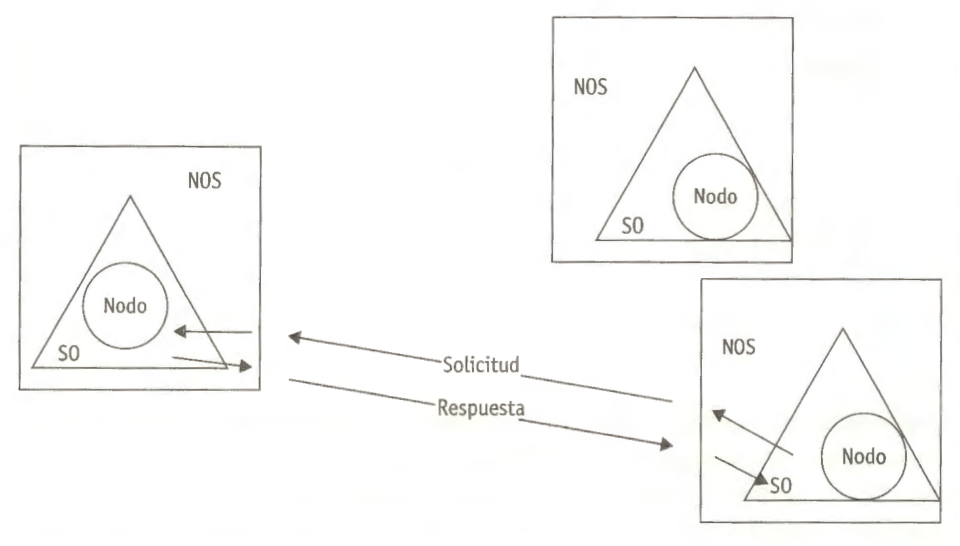
\includegraphics[width=\linewidth, keepaspectratio]{media/t06/comparativaArquitecturaNosDos_1.png}
    \end{minipage}\hfill
    \begin{minipage}[b]{0.48\textwidth}
        \centering
        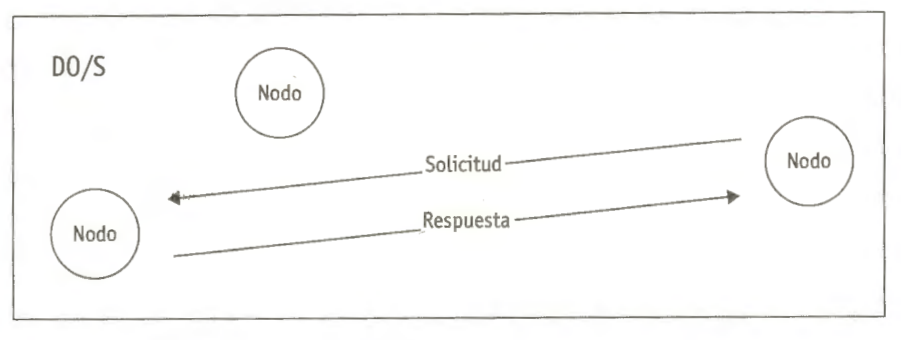
\includegraphics[width=\linewidth, keepaspectratio]{media/t06/comparativaArquitecturaNosDos_2.png}
    \end{minipage}
    \caption{Comparación estructural entre el modelo desacoplado de sistema operativo de red (NOS, izquierda) y el modelo integrado de sistema operativo distribuido (DO/S, derecha) \parencite[\S 10, pp.\ 319--320]{mchoes2011sistemas}.}
    \label{fig:comparativaArquitecturaNosDos}
\end{figure}

Como ilustra la Img.~\ref{fig:comparativaArquitecturaNosDos}, el DO/S asume el control directo del hardware en cada nodo. En la administración de procesos, el planificador global distribuye la carga algorítmicamente mediante migración de procesos, transfiriendo de forma transparente el bloque de control del proceso (PCB), su contexto de ejecución y descriptores abiertos hacia los procesadores con menor carga \parencite[\S 16.2, p.\ 563]{silberschatz2006fundamentos}. En la gestión de memoria, implementa memoria compartida distribuida (\textit{distributed shared memory}, DSM), donde los fallos de página sobre direcciones remotas activan transferencias de bloques en red sin intervención del hilo solicitante \parencite[\S 10, pp.\ 321--322]{mchoes2011sistemas}.

\subsection{Dimensiones de transparencia y características esenciales}
\label{sec:dimensionesTransparencia}

El fin primordial del DO/S es la transparencia. El Modelo de Referencia para Procesamiento Distribuido Abierto (RM-ODP, ISO/IEC 10746) sistematiza ocho dimensiones de transparencia cardinales \parencite[\S 17.2, pp.\ 786--787]{deitel2004operating}:
\begin{enumerate}[noitemsep, topsep=2pt, parsep=0pt]
    \item \textbf{Acceso (\textit{access transparency}):} Oculta disparidades de protocolos y representaciones de datos (\textit{endianness}, formatos de coma flotante) entre arquitecturas heterogéneas.
    \item \textbf{Ubicación (\textit{location transparency}):} Oculta la localización física de los recursos; las entidades se direccionan mediante nombres lógicos globales sin conocer el host anfitrión.
    \item \textbf{Migración (\textit{migration transparency}):} Permite transferir recursos o procesos entre nodos sin suspender la operación de los clientes asociados.
    \item \textbf{Reubicación (\textit{relocation transparency}):} Enmascara la relocalización de un componente mientras éste se encuentra siendo accedido concurrentemente por otros objetos.
    \item \textbf{Replicación (\textit{replication transparency}):} Mantiene copias redundantes para alta disponibilidad y desempeño, mostrándolas como una única instancia consistente.
    \item \textbf{Concurrencia (\textit{concurrency transparency}):} Permite el acceso simultáneo a recursos compartidos garantizando consistencia sin interferencias destructivas.
    \item \textbf{Fallos (\textit{failure transparency}):} Oculta la interrupción de nodos o enlaces de comunicación mediante puntos de control (\textit{checkpointing}) y conmutación por fallo.
    \item \textbf{Persistencia (\textit{persistence transparency}):} Enmascara si una entidad reside en la memoria volátil o en almacenamiento persistente secundario.
\end{enumerate}

Complementariamente, el sistema exhibe cuatro propiedades indispensables: \textbf{escalabilidad} para soportar crecimiento en nodos y carga sin degradación estructural; \textbf{heterogeneidad} en procesadores y redes mediante capas de \textit{middleware}; \textbf{tolerancia a fallos} ante particiones de red; y \textbf{sincronización lógica} fundamentada en marcas de tiempo causales (relojes de Lamport) ante la ausencia de un reloj físico unificado \parencite[\S 18.1, p.\ 605]{silberschatz2006fundamentos}.

\subsection{Análisis comparativo: ventajas, desventajas y compromisos de diseño}
\label{sec:analisisComparativoNosDos}

La adopción de esquemas distribuidos frente a entornos centralizados responde a ventajas operativas concretas \parencite[\S 16.1, pp.\ 557--559]{silberschatz2006fundamentos}: compartición global de periféricos y datos masivos; aceleración del cómputo mediante paralelismo y balanceo dinámico de subprocesos; resiliencia operativa ante caídas individuales de nodos; y soporte nativo para llamadas a procedimientos remotos (\textit{remote procedure calls}, RPC).

Sin embargo, estos beneficios introducen severos compromisos de diseño (\textit{trade-offs}) \parencite[\S 17.2, p.\ 788]{deitel2004operating}: la sobrecarga y latencia inherente al paso de mensajes por red en lugar de buses locales; la extrema complejidad en la detección de interbloqueos distribuidos (\textit{deadlocks}); y una superficie de ataque significativamente ampliada, donde la seguridad perimetral, la autenticación mutua y el cifrado de canales devienen imperativos.

En la Tabla~\ref{tab:comparativaNosDos} se sintetizan las diferencias arquitectónicas entre ambos modelos.

\begin{table}[H]
\centering
\small
\renewcommand{\arraystretch}{1.15}
\renewcommand{\tabularxcolumn}[1]{m{#1}}
\setlength{\emergencystretch}{1.5em}
\caption{Comparación técnica entre sistemas operativos de red (NOS) y sistemas operativos distribuidos (DO/S).}
\label{tab:comparativaNosDos}
\begin{tabularx}{\textwidth}{>{\centering\arraybackslash}m{3.1cm} X X}
\toprule
\textbf{Criterio técnico} & \textbf{Sistema operativo de red (NOS)} & \textbf{Sistema operativo distribuido (DO/S)} \\
\midrule
\textbf{Dominio de recursos} & Recursos pertenecientes a nodos locales bajo soberanía de su núcleo anfitrión \parencite[\S 10, p.\ 320]{mchoes2011sistemas}. & Recursos pertenecientes a un dominio global unificado gobernado por el DO/S. \\
\addlinespace
\textbf{Autonomía de nodos} & Máxima; los hosts conservan independencia operativa y ejecución desacoplada. & Reducida; nodos estrechamente interdependientes subordinados al planificador global. \\
\addlinespace
\textbf{Transparencia} & Baja; el usuario conoce la ubicación de servidores y protocolos de conexión \parencite[\S 17.2, p.\ 787]{deitel2004operating}. & Total; provee una imagen de sistema único (SSI) que oculta la red física. \\
\addlinespace
\textbf{Memoria y procesos} & Gestión puramente local; no existe migración de procesos ni memoria compartida nativa. & Gestión de memoria compartida distribuida (DSM) y migración automática de procesos. \\
\addlinespace
\textbf{Comunicaciones} & Comunicación explícita mediante \textit{sockets}, clientes dedicados y protocolos de red (NFS, SSH). & Comunicación transparente vía paso de mensajes del núcleo y abstracciones RPC. \\
\addlinespace
\textbf{Tolerancia a fallos} & Resuelta a nivel de aplicación mediante configuraciones de alta disponibilidad externas. & Integrada nativamente en el núcleo con detección de fallos y reconfiguración dinámica. \\
\addlinespace
\textbf{Complejidad} & Moderada; construido como módulos de red sobre sistemas operativos comerciales. & Muy elevada; exige núcleos especializados y sincronización formal estricta. \\
\bottomrule
\end{tabularx}
\end{table}

Históricamente, la elevada complejidad de los DO/S puros relegó sus implementaciones completas (Amoeba, Plan 9, Sprite) a la esfera investigativa. La industria consolidó un modelo híbrido pragmático: sistemas operativos de red estandarizados como base de ejecución de nodo (Linux y Windows Server), sobre los cuales plataformas de orquestación y computación en la nube (Kubernetes, OpenStack) proveen las capas de transparencia, migración y balanceo requeridas sin renunciar a la robustez de los núcleos comerciales.

\section{Taxonomía de servicios y arquitecturas de servidores}
\label{sec:taxonomiaServiciosServidores}

El despliegue de soluciones informáticas distribuidas descansa sobre el desacoplamiento de funciones computacionales entre entidades colaboradoras. En este entorno, la provisión de capacidades de procesamiento, almacenamiento y comunicaciones se articula a través de arquitecturas estructuradas donde procesos especializados atienden requerimientos concurrentes provenientes de múltiples orígenes a través de la infraestructura de red.

\subsection{Modelos cliente-servidor y paradigmas de comunicación distribuida}
\label{sec:modelosClienteServidor}

El modelo cliente-servidor constituye la arquitectura dominante en los sistemas distribuidos contemporáneos. Se fundamenta en una asimetría funcional estricta: el proceso \textbf{cliente} inicia la interacción solicitando la ejecución de una tarea o el acceso a un dato, mientras que el proceso \textbf{servidor} permanece a la escucha pasiva en un puerto de red predefinido, atiende la petición, procesa la transacción y devuelve un mensaje de respuesta al emisor \parencite[\S 1.12, p.\ 26]{silberschatz2006fundamentos}. 

Desde una perspectiva analítica de ingeniería de software y sistemas operativos, cualquier aplicación distribuida descompone su funcionalidad en tres capas estructurales \parencite[\S 18.1, pp.\ 18-5--18-6]{stallings2018operating}:
\begin{enumerate}[noitemsep, topsep=2pt, parsep=0pt]
    \item \textbf{Capa de presentación (\textit{presentation logic}):} Responsable de la interacción con el usuario humano o con sistemas externos, formateando las pantallas, capturando eventos de entrada y desplegando los datos de salida.
    \item \textbf{Capa de lógica de aplicación (\textit{application logic}):} Contiene las reglas operativas, algoritmos de cálculo, transformaciones de negocio y validaciones que definen el comportamiento medular del sistema.
    \item \textbf{Capa de gestión de datos (\textit{data management}):} Encargada del almacenamiento físico persistente, indexación, ejecución de consultas estructuradas, control de transacciones concurrentes y preservación de la integridad referencial.
\end{enumerate}

La delimitación de la frontera física donde se ejecutan estas capas sobre la infraestructura de red determina el espectro de particionamiento arquitectónico \parencite[\S 18.1, pp.\ 18-6--18-9]{stallings2018operating}:
\begin{itemize}[noitemsep, topsep=2pt, parsep=0pt]
    \item \textbf{Procesamiento basado en host (\textit{host-based processing}):} Modelo centralizado tradicional donde las tres capas residen íntegramente en el servidor central; la estación del usuario actúa como terminal pasiva limitada a pintar caracteres en pantalla.
    \item \textbf{Procesamiento basado en servidor (cliente ligero o \textit{thin client}):} La estación cliente ejecuta exclusivamente la presentación visual básica, delegando toda la lógica de aplicación y el acceso a datos en servidores centrales con alta potencia de cómputo.
    \item \textbf{Procesamiento basado en cliente (cliente pesado o \textit{fat client}):} La presentación y la lógica de aplicación completa se compilan y ejecutan en la máquina de trabajo del usuario; el servidor se restringe a actuar como motor de base de datos o almacén de ficheros compartidos.
    \item \textbf{Arquitecturas multinivel (tres o más capas):} Desacoplan físicamente cada capa en plataformas independientes (interfaz en navegador web o cliente móvil, lógica de negocio en servidores de aplicaciones y datos en clústeres de almacenamiento), optimizando la escalabilidad y el mantenimiento modular.
\end{itemize}

Para articular la interacción entre estos niveles, los sistemas operativos y las capas de software intermedio implementan diversos paradigmas de comunicación distribuida \parencite[\S 17.3, pp.\ 788--793]{deitel2004operating}:
\begin{itemize}[noitemsep, topsep=2pt, parsep=0pt]
    \item \textbf{Paso de mensajes mediante puntos finales (sockets):} Primitiva de bajo nivel basada en descriptores de red que permite a dos procesos intercambiar flujos de bytes (orientados a conexión con TCP) o datagramas discretos (sin conexión con UDP). Requiere que el programador diseñe explícitamente el protocolo de formateo y serialización de mensajes.
    \item \textbf{Llamadas a procedimientos remotos (RPC):} Abstracción de alto nivel que permite invocar funciones situadas en una máquina remota empleando la misma sintaxis semántica de una llamada local. El mecanismo depende de un talón de cliente (\textit{client stub}) que empaqueta los argumentos (\textit{marshaling}) y los transmite por la red, y un talón de servidor (\textit{server stub}) que los desempaqueta (\textit{unmarshaling}), ejecuta la rutina y devuelve el resultado, garantizando transparencia sintáctica \parencite[\S 18.3, pp.\ 18-16--18-18]{stallings2018operating}.
    \item \textbf{Invocación de métodos remotos (RMI) y arquitecturas orientadas a servicios:} Extensión del paradigma RPC al modelo orientado a objetos (como Java RMI), que posibilita invocar métodos pasando referencias a objetos distribuidos, evolucionando hacia servicios web desacoplados basados en protocolos de transporte estándar (REST sobre HTTP/HTTPS, gRPC con búferes de protocolo).
    \item \textbf{Modelo entre iguales (\textit{peer-to-peer}, P2P):} Paradigma simétrico donde desaparece la división estática entre cliente y servidor. Cada nodo (\textit{peer}) posee idénticas capacidades funcionales, actuando simultáneamente como cliente que consume recursos y servidor que proporciona almacenamiento o capacidad de cálculo a la red, eliminando cuellos de botella centralizados \parencite[\S 1.12, pp.\ 27--28]{silberschatz2006fundamentos}.
\end{itemize}

\subsection{Clasificación funcional de servidores en redes corporativas}
\label{sec:clasificacionFuncionalServidores}

En los entornos de producción modernos, la especialización funcional de las máquinas servidoras permite garantizar el aislamiento de procesos, maximizar la eficiencia en el aprovechamiento de recursos físicos (CPU, memoria RAM, buses de almacenamiento y ancho de banda de red) y consolidar directivas de seguridad uniformes. Conforme a las demandas de infraestructura y a los servicios que proveen a los sistemas operativos clientes, los servidores se clasifican técnicamente en las siguientes categorías cardinales:

\begin{enumerate}[noitemsep, topsep=1pt, parsep=0pt]
    \item \textbf{Infraestructura básica y direccionamiento:} Proveen resolución de nombres y parámetros de red en capas 3 y 4. Incluyen servidores DNS (traducción jerárquica de nombres a direcciones IP) y servidores DHCP (concesión y renovación automática de direcciones IP, máscaras y pasarelas).
    \item \textbf{Almacenamiento y archivos:} Abstraen unidades secundarias mediante sistemas de archivos de red (NFS, SMB/CIFS) o almacenamiento en bloque (iSCSI, Fibre Channel). Implementan control de concurrencia, cuotas, listas ACL, instantáneas (\textit{snapshots}) y arreglos RAID \parencite[\S 10, pp.\ 325--326]{mchoes2011sistemas}.
    \item \textbf{Gestión de impresión:} Coordinan el acceso concurrente a periféricos de salida mediante colas en disco (\textit{spooling}) y traducción de flujos (PDF, PostScript, PCL) usando protocolos estándar como IPP o LPD/LPR.
    \item \textbf{Directorio, identidad y autenticación:} Centralizan credenciales, perfiles y directivas de seguridad corporativas mediante LDAP, Kerberos (emisión de boletos de autenticación mutua) o RADIUS (autorización centralizada de accesos de red).
    \item \textbf{Seguridad perimetral y enrutamiento:} Regulan el flujo entre zonas de red dispares mediante cortafuegos con seguimiento de estados (\textit{stateful inspection}), traducción NAT para aislar direccionamiento privado (RFC 1918) y servidores proxy con almacenamiento en caché e inspección de contenido.
    \item \textbf{Aplicaciones y bases de datos:} Procesan la lógica de negocio y transacciones persistentes. Integran servidores web (Apache, Nginx), motores de ejecución (Node.js, PHP-FPM) y sistemas RDBMS (PostgreSQL, MariaDB, Oracle) bajo garantías ACID.
    \item \textbf{Acceso remoto y comunicaciones (RAS):} Proveen conectividad segura a clientes remotos hacia la LAN interna mediante túneles cifrados de red privada virtual (VPN) basados en protocolos como IPsec, OpenVPN o WireGuard.
\end{enumerate}

Para sintetizar la articulación funcional de estos componentes dentro de la infraestructura tecnológica, en la Tabla~\ref{tab:clasificacionServidores} se presenta una matriz comparativa que clasifica los servidores según su rol operativo, los protocolos cardinales involucrados y su impacto en la administración de recursos del sistema operativo anfitrión.

\begin{table}[H]
\centering
\small
\renewcommand{\arraystretch}{1.15}
\renewcommand{\tabularxcolumn}[1]{m{#1}}
\setlength{\emergencystretch}{1.5em}
\caption{Clasificación funcional de servidores en redes corporativas.}
\label{tab:clasificacionServidores}
\begin{tabularx}{\textwidth}{>{\centering\arraybackslash}m{3.1cm} X X}
\toprule
\textbf{Categoría de servidor} & \textbf{Protocolos y estándares cardinales} & \textbf{Recursos críticos del sistema operativo} \\
\midrule
\textbf{Infraestructura de red} & DNS (puerto 53 UDP/TCP), DHCP (puertos 67/68 UDP), NTP, IPAM. & Baja latencia en resolución de sockets, estabilidad en interfaces de red e integridad en tablas de concesiones. \\
\addlinespace
\textbf{Almacenamiento y archivos} & NFSv4 (puerto 2049 TCP), SMB/CIFS (puerto 445 TCP), iSCSI (puerto 3260 TCP). & Búferes de caché en memoria de páginas, alto rendimiento de E/S en disco (\textit{IOPS}) y gestión de inodos/ACL. \\
\addlinespace
\textbf{Gestión de impresión} & IPP (puerto 631 TCP), LPD/LPR (puerto 515 TCP), filtros PPD/Ghostscript. & Espacio de almacenamiento temporal para colas de ficheros en disco (\textit{spool}) y aislamiento de filtros de rasterización. \\
\addlinespace
\textbf{Directorio y autenticación} & LDAP/LDAPS (puertos 389/636 TCP), Kerberos (puerto 88 UDP/TCP), RADIUS (puertos 1812/1813 UDP). & Sincronización estricta de relojes lógicos, cifrado en memoria y rapidez de consulta en estructuras arbóreas indexadas. \\
\addlinespace
\textbf{Seguridad y perímetro} & Filtrado \textit{netfilter}/nftables, NAT (RFC 3022), HTTP/SOCKS en proxies (Squid). & Eficiencia del núcleo en inspección de paquetes en anillo 0, tablas de seguimiento de conexiones y memoria de caché. \\
\addlinespace
\textbf{Aplicaciones y datos} & HTTP/HTTPS (puertos 80/443 TCP), FastCGI, SQL (PostgreSQL, MariaDB). & Asignación masiva de memoria RAM compartida para cachés de base de datos, múltiples hilos de CPU y descriptores abiertos. \\
\addlinespace
\textbf{Acceso remoto (RAS)} & IPsec (IKEv2, puertos 500/4500 UDP), OpenVPN (puerto 1194 UDP), WireGuard (UDP). & Interrupciones por aceleración criptográfica (AES-NI), interfaces de red virtuales (TUN/TAP) y control de enrutamiento. \\
\bottomrule
\end{tabularx}
\end{table}

Esta segmentación funcional evidencia que un servidor contemporáneo no se define primordialmente por su arquitectura física de hardware, sino por la naturaleza de los demonios y servicios que ejecuta en su espacio de usuario y en su núcleo, así como por las políticas de asignación de recursos que el sistema operativo implementa para garantizar su disponibilidad y resiliencia en la red.

\section{Sistemas operativos orientados a servidores}
\label{sec:sistemasOperativosServidores}

El funcionamiento continuo de una infraestructura de red corporativa depende de la estabilidad, seguridad y rendimiento del sistema operativo que gobierna el hardware de cada estación servidora. A diferencia de las distribuciones diseñadas para estaciones de trabajo cliente o consumo personal, un sistema operativo para servidor está especializado en gestionar concurrencia masiva, maximizar el aprovechamiento de los recursos físicos de cálculo y mitigar cualquier evento que comprometa la disponibilidad del servicio.

\subsection{Arquitectura y especialización de sistemas operativos para servidor}
\label{sec:arquitecturaEspecializacionServidores}

La distinción entre un sistema operativo de escritorio (\textit{desktop}) y uno orientado a servidores no reside necesariamente en las llamadas al sistema fundamentales, sino en las políticas de configuración del núcleo, la asignación de memoria, la planificación de la CPU y la omisión deliberada de subsistemas innecesarios:
\begin{enumerate}[noitemsep, topsep=2pt, parsep=0pt]
    \item \textbf{Políticas del planificador de la CPU:} En un sistema de escritorio, el planificador prioriza la latencia de respuesta interactiva para que las aplicaciones de la interfaz gráfica respondan inmediatamente a eventos de teclado y ratón. En contraste, un núcleo de servidor optimiza el rendimiento global (\textit{throughput}) y la equidad en el tiempo de procesamiento, minimizando los cambios de contexto costosos entre los miles de hilos de trabajo de bases de datos o servidores web concurrentes \parencite[\S 18.1, pp.\ 18-3--18-4]{stallings2018operating}.
    \item \textbf{Gestión de memoria física y caché de páginas:} Un servidor dedica la mayor parte de su memoria RAM a la caché de páginas del núcleo (\textit{page cache}) para acelerar las lecturas y escrituras en disco. Además, ajusta la agresividad del intercambio de memoria (\textit{swappiness}) para evitar la expulsión prematura de páginas activas de procesos transaccionales hacia el almacenamiento secundario.
    \item \textbf{Subsistema de red y colas de interrupción:} Los servidores implementan técnicas de alto rendimiento como el escalado lateral de recepción (RSS, \textit{Receive Side Scaling}) para distribuir el procesamiento de paquetes entrantes entre múltiples núcleos físicos de CPU, combinadas con llamadas asíncronas no bloqueantes de multiplexación de descriptores (como \texttt{epoll} en Linux, \texttt{kqueue} en BSD y puertos de finalización de E/S o \textit{IOCP} en Windows NT), permitiendo atender decenas de miles de conexiones simultáneas por proceso.
    \item \textbf{Confiabilidad del almacenamiento secundario:} Incorporan soporte nativo para sistemas de archivos transaccionales avanzados que implementan comprobación de redundancia de datos (\textit{checksumming}), instantáneas de volumen (snapshots), compresión en línea y administración de volúmenes lógicos con tolerancia a fallos mediante arreglos redundantes de discos independientes (RAID) por hardware o software.
    \item \textbf{Minimización de superficie de ataque:} Los sistemas de servidor prescinden por defecto de servidores gráficos (X11 o Wayland) y entornos de escritorio, operando exclusivamente en modo terminal de línea de comandos (CLI) administrada por SSH o interfaces remotas declarativas, lo que reduce drásticamente el consumo de memoria en reposo y cierra vectores de vulnerabilidad.
\end{enumerate}

\subsection{Estudio técnico y comparativo de diez plataformas de servidor}
\label{sec:estudioDiezPlataformas}

A continuación se analizan diez plataformas representativas empleadas en la industria, detallando su arquitectura de núcleo, mecanismos de seguridad, subsistemas de almacenamiento y áreas cardinales de aplicación.

\subsubsection{Microsoft Windows Server}
Basado en la arquitectura del núcleo Windows NT (núcleo híbrido), desacopla el hardware mediante la capa HAL y ejecuta sus subsistemas ejecutivos en anillo 0 \parencite{microsoftWindowsServer}. Es el pilar de redes corporativas mediante Active Directory (AD DS), integrando autenticación Kerberos, directivas de grupo (GPO), virtualización Hyper-V y sistemas de archivos NTFS y ReFS (\textit{Resilient File System}), administrado mediante PowerShell y Windows Admin Center.

\subsubsection{Red Hat Enterprise Linux (RHEL)}
Estándar comercial de referencia para entornos de misión crítica con ciclo de vida extendido de diez años. Basado en un núcleo monolítico modular de Linux, destaca por la integración nativa de SELinux (\textit{Security-Enhanced Linux}) en modo forzoso por defecto (control de acceso obligatorio, MAC) \parencite{redhatRhel}, gestor DNF/RPM, sistema de archivos transaccional XFS y despliegue de contenedores OCI mediante Podman y Buildah.

\subsubsection{Debian GNU/Linux}
Sistema operativo universal sustentado en gobernanza comunitaria abierta y rigor técnico extremo en su rama estable \parencite{debianBookworm}. Utiliza el sistema de paquetes APT (\texttt{dpkg}), ofrece un consumo de memoria basal mínimo en modo servidor y garantiza máxima previsibilidad operativa, consolidándose como la base troncal de múltiples distribuciones industriales.

\subsubsection{Ubuntu Server}
Variante empresarial mantenida por Canonical derivada de Debian con ciclo predecible de versiones LTS cada dos años y hasta diez años de soporte extendido \parencite{canonical2024server}. Se encuentra optimizada para cómputo en la nube e infraestructuras de microservicios, integrando configuración de red con Netplan, ZFS en Linux, paquetes aislados Snap y aprovisionamiento desatendido con MAAS.

\subsubsection{SUSE Linux Enterprise Server (SLES)}
Distribución corporativa diseñada para cómputo intensivo y centros de datos de misión crítica, certificada para bases de datos en memoria SAP HANA \parencite{suseSles}. Integra la herramienta centralizada de administración YaST, paquetería RPM con Zypper y el sistema de archivos Btrfs con instantáneas automáticas Snapper para recuperación inmediata ante actualizaciones.

\subsubsection{FreeBSD}
Sistema operativo UNIX descendiente directo del código de investigación BSD de UC Berkeley, que desarrolla su núcleo modular y espacio de usuario como un sistema unificado \parencite{freebsdRelnotes}. Sobresale por su pila de red de muy alto rendimiento, almacenamiento de 128 bits OpenZFS nativo con autorreparación y virtualización ligera mediante jaulas (\textit{FreeBSD Jails}) para aislamiento sin hipervisor.

\subsubsection{Oracle Solaris / illumos}
Sistema operativo UNIX SVR4 certificado, diseñado para servidores multiprocesador masivos \parencite{oracleSolaris}. Plataforma pionera que introdujo el sistema transaccional ZFS con sumas de verificación, el marco de observabilidad DTrace, zonas de aislamiento (\textit{Solaris Zones}) y el gestor tolerante a fallos SMF, tecnologías cuyo desarrollo abierto continúa en el proyecto illumos.

\subsubsection{OpenBSD}
Sistema de la familia BSD enfocado prioritariamente en máxima seguridad proactiva y auditoría técnica permanente del código fuente \parencite{openbsdProject}. Creador de OpenSSH y del cortafuegos Packet Filter (PF), implementa mitigaciones de memoria avanzadas en su núcleo (W\^{}X, ASLR aleatorio) y llamadas restrictivas \texttt{pledge} y \texttt{unveil} para confinamiento estricto de procesos.

\subsubsection{Rocky Linux / AlmaLinux}
Distribuciones comunitarias surgidas para preservar la compatibilidad binaria 1:1 con RHEL tras el cambio de enfoque de CentOS hacia CentOS Stream \parencite{rockyLinux}. Proporcionan la robustez, el gestor DNF/RPM, el confinamiento de SELinux y el soporte de aplicaciones corporativas de grado RHEL de manera libre y sin costos de licenciamiento.

\subsubsection{VMware ESXi}
Hipervisor de tipo 1 (\textit{bare-metal}) especializado en la virtualización de servidores en centros de datos, ejecutándose directamente sobre el silicio del equipo sin un sistema operativo anfitrión intermedio \parencite{vmwareEsxi}. Su núcleo propietario VMkernel administra directamente vCPUs, compresión y deduplicación de memoria RAM, y almacenamiento VMFS, maximizando la densidad de consolidación virtual.

\subsubsection{Matriz comparativa de sistemas operativos de servidor}
Para estructurar las diferencias arquitectónicas y operativas de estas diez plataformas, en la Tabla~\ref{tab:comparativaDiezSistemas} se sintetiza su diseño interno, mecanismos de aislamiento y entornos de aplicación principales.

\begin{table}[H]
\centering
\scriptsize
\renewcommand{\arraystretch}{1.1}
\renewcommand{\tabularxcolumn}[1]{m{#1}}
\setlength{\emergencystretch}{1.5em}
\caption{Comparación técnica de diez plataformas de sistema operativo orientadas a servidores.}
\label{tab:comparativaDiezSistemas}
\begin{tabularx}{\textwidth}{>{\centering\arraybackslash}m{2.3cm} X X X X}
\toprule
\textbf{Sistema operativo} & \textbf{Núcleo y familia} & \textbf{Almacenamiento nativo} & \textbf{Aislamiento y seguridad} & \textbf{Nicho corporativo principal} \\
\midrule
\textbf{Windows Server} & Núcleo híbrido (familia Windows NT). & NTFS, ReFS, espacios de almacenamiento directo. & Listas ACL de Windows, aislamiento Hyper-V, directivas GPO. & Servicios de directorio Active Directory, aplicaciones .NET, servidores corporativos Windows. \\
\addlinespace
\textbf{RHEL} & Monolítico modular (GNU/Linux). & XFS (predeterminado), ext4, LVM. & SELinux forzoso (MAC), cortafuegos \textit{firewalld}, contenedores Podman. & Cargas de misión crítica corporativa, centros de datos empresariales y nubes privadas. \\
\addlinespace
\textbf{Debian} & Monolítico modular (GNU/Linux). & ext4, XFS, Btrfs, soporte ZFS. & Permisos POSIX, AppArmor/SELinux configurable, paquetería APT estricta. & Infraestructura de servidores web de alta estabilidad, servicios comunitarios y base de sistemas. \\
\addlinespace
\textbf{Ubuntu Server} & Monolítico modular (GNU/Linux). & ext4, ZFS en Linux, LVM. & Perfiles AppArmor, confinamiento Snap, actualizaciones automáticas de seguridad. & Nube pública (AWS, Azure, GCP), entornos de contenedores Kubernetes y microservicios. \\
\addlinespace
\textbf{SLES} & Monolítico modular (GNU/Linux). & Btrfs con instantáneas Snapper, XFS. & AppArmor, configuración integral YaST, alta disponibilidad con clúster Pacemaker. & Plataformas ERP empresariales, bases de datos SAP HANA y grandes clústeres de computación. \\
\addlinespace
\textbf{FreeBSD} & Monolítico modular (UNIX/BSD). & OpenZFS (128 bits con autorreparación), UFS2. & Jaulas (\textit{Jails}) para virtualización ligera de SO, cortafuegos Packet Filter (PF). & Infraestructuras de red de alta tasa de transferencia, enrutadores perimetrales y servidores ZFS. \\
\addlinespace
\textbf{Solaris / illumos} & Monolítico modular simétrico (UNIX SVR4). & ZFS nativo con compresión e instantáneas. & Zonas de aislamiento (Solaris Zones), observabilidad DTrace, RBAC. & Servidores multiprocesador masivos, bases de datos Oracle de alto rendimiento y almacenamiento ZFS. \\
\addlinespace
\textbf{OpenBSD} & Monolítico (UNIX/BSD). & FFS2 (\textit{Fast File System}), softupdates. & Mitigaciones W\^{}X, ASLR aleatorio, llamadas \texttt{pledge}/\texttt{unveil}, cortafuegos PF. & Cortafuegos perimetrales, concentradores de VPN, servidores DNS/BGP y entornos de alta seguridad. \\
\addlinespace
\textbf{Rocky / AlmaLinux} & Monolítico modular (GNU/Linux). & XFS, ext4, LVM estructurado. & SELinux en modo forzoso, compatibilidad binaria 1:1 con directivas RHEL. & Reemplazo corporativo de CentOS, entornos universitarios y centros de cómputo sin costo de suscripción. \\
\addlinespace
\textbf{VMware ESXi} & Micronúcleo propietario especializado (VMkernel). & VMFS (\textit{Virtual Machine File System}), vSAN. & Aislamiento de hardware en anillo 0, segmentación de vSwitch y cifrado de VM. & Consolidación masiva de servidores virtuales en centros de datos corporativos (hipervisor tipo 1). \\
\bottomrule
\end{tabularx}
\end{table}

\section{Servidores de conectividad, enrutamiento y seguridad perimetral}
\label{sec:servidoresConectividadSeguridad}

La operación continua de una red corporativa demanda mecanismos de control de tráfico en las capas de red, transporte y aplicación. Los servidores de conectividad y seguridad perimetral regulan los flujos de paquetes que transitan entre segmentos internos y redes públicas desconfiadas, mitigando vectores de ataque, optimizando el espacio de direccionamiento y dinamizando la asignación de parámetros de red.

\subsection{Servidores de traducción de direcciones de red (NAT)}
\label{sec:servidoresNat}

La traducción de direcciones de red (\textit{Network Address Translation}, NAT), formalizada en el RFC 3022, permite a un enrutador o pasarela perimetral modificar en tránsito las cabeceras de los paquetes IP, mapeando direcciones privadas no enrutables (RFC 1918) a direcciones IP públicas globalmente enrutables \parencite[\S 1, pp.\ 1--3]{rfc3022}. Esta tecnología surgió para mitigar el agotamiento de direcciones IPv4 de 32 bits, consolidando a la vez un aislamiento estructural que oculta la topología interna.

En el núcleo del sistema operativo anfitrión, el módulo NAT opera en anillo 0 interceptando los paquetes en los ganchos de preenrutamiento (\textit{prerouting}) o postenrutamiento (\textit{postrouting}). Se implementa bajo tres esquemas operativos:
\begin{itemize}[noitemsep, topsep=1pt, parsep=0pt]
    \item \textbf{NAT estático:} Correspondencia biunívoca permanente (1:1) entre una IP privada y una pública para exponer servidores internos sin revelar su subred real.
    \item \textbf{NAT dinámico:} Asignación temporal de una dirección pública extraída de un grupo (\textit{pool}) reservado mientras dure la sesión del host.
    \item \textbf{Traducción de direcciones y puertos (NAPT/PAT):} Esquema masivo donde múltiples hosts internos comparten una sola IP pública mediante sobrecarga de puertos en la capa de transporte \parencite[\S 4, pp.\ 6--8]{rfc3022}, reescribiendo la IP origen y sustituyendo el puerto efímero local por uno asignado dinámicamente en el servidor.
\end{itemize}

El seguimiento de conexiones se sustenta en una tabla en la memoria del núcleo (módulo \texttt{nf\_conntrack} en Linux), que indexa la tupla de cinco elementos: IP origen, puerto origen, IP destino, puerto destino y protocolo. Al retornar el tráfico, el núcleo sustituye la cabecera, recalcula las sumas de comprobación (\textit{checksums}) de IP y TCP/UDP en tiempo real y conmuta el paquete hacia la subred local. Para protocolos de capa 7 que incrustan direcciones IP en su carga útil (como FTP activo o SIP), el núcleo invoca pasarelas a nivel de aplicación (ALG, \textit{Application Layer Gateway}) que reescriben los campos internos de señalización.

\subsection{Servidores de filtrado y cortafuegos (Firewall)}
\label{sec:servidoresFirewall}

Un cortafuegos (\textit{firewall}) aplica directivas de control de acceso entre zonas de confianza dispares, inspeccionando el tráfico bidireccional para autorizar, rechazar o descartar tramas conforme a políticas formales \parencite[\S 19.3, pp.\ 942--944]{deitel2004operating}. Arquitectónicamente, se diferencian tres niveles de inspección:
\begin{enumerate}[noitemsep, topsep=1pt, parsep=0pt]
    \item \textbf{Filtrado sin estado (\textit{stateless}):} Examina cabeceras aisladas en capas 3 y 4 (IP origen/destino, puerto y banderas TCP como SYN, ACK o RST) sin memoria de flujos previos, siendo vulnerable a suplantaciones de identidad.
    \item \textbf{Inspección con estado (\textit{stateful packet inspection}, SPI):} Modela los flujos mediante máquinas de estado finito en el núcleo. Al validar el saludo de tres vías de TCP, cataloga la conexión como \texttt{NEW} y luego \texttt{ESTABLISHED} \parencite[\S 19.3, p.\ 943]{deitel2004operating}; los paquetes de respuesta válidos se conmutan de forma inmediata y el tráfico no solicitado se descarta.
    \item \textbf{Cortafuegos de aplicación (WAF / NGFW):} Reensambla flujos en capa 7 para analizar la semántica de protocolos web (HTTP/HTTPS, DNS), ejecutando inspección profunda de paquetes (\textit{Deep Packet Inspection}, DPI) contra inyecciones y anomalías de carga útil.
\end{enumerate}

En el espacio de núcleo de Linux, el marco de trabajo netfilter provee los puntos de enganche \texttt{PREROUTING}, \texttt{INPUT}, \texttt{FORWARD}, \texttt{OUTPUT} y \texttt{POSTROUTING}, operados por el subsistema moderno \texttt{nftables}, que ejecuta las reglas como código de máquina virtual de bytes en anillo 0 para minimizar la sobrecarga de interrupciones de CPU. En entornos BSD, Packet Filter (PF) ejecuta normalización de tráfico (\textit{scrubbing}), resolviendo la desfragmentación de paquetes y el saneamiento de banderas TCP antes de la evaluación de políticas.

\subsection{Servidores de configuración dinámica de direcciones (DHCP)}
\label{sec:servidoresDhcp}

El protocolo de configuración dinámica de host (\textit{Dynamic Host Configuration Protocol}, DHCP), especificado en el RFC 2131, automatiza la asignación centralizada de direccionamiento y parámetros de red a clientes locales, evitando colisiones por duplicidad de IP \parencite[\S 1, pp.\ 1--4]{rfc2131}.

La negociación de parámetros opera en espacio de usuario sobre sockets UDP (puertos 67 en el servidor y 68 en el cliente) mediante el ciclo DORA de cuatro fases:
\begin{enumerate}[noitemsep, topsep=1pt, parsep=0pt]
    \item \textbf{DHCPDISCOVER:} Difusión masiva (\textit{broadcast} en capa 2 \texttt{ff:ff:ff:ff:ff:ff} y capa 3 \texttt{255.255.255.255}) emitida por el cliente con su dirección MAC física para localizar servidores disponibles.
    \item \textbf{DHCPOFFER:} Los servidores receptores seleccionan una IP libre de su ámbito (\textit{scope}) y responden con una oferta que detalla la IP propuesta, la máscara de subred y el tiempo de concesión (\textit{lease time}).
    \item \textbf{DHCPREQUEST:} El cliente selecciona formalmente una oferta y difunde su aceptación para notificar a los servidores y liberar las reservas descartadas.
    \item \textbf{DHCPACK:} El servidor seleccionado confirma la concesión e inserta las opciones RFC 2132: pasarela predeterminada (\textit{default gateway}), servidores DNS, sufijo de búsqueda y servidores NTP \parencite[\S 3.1, pp.\ 13--16]{rfc2131}.
\end{enumerate}

El cliente gestiona la vida del alquiler con dos temporizadores: T1 (al 50\,\% del tiempo, renegociación unicast directa) y T2 (al 87.5\,\% del tiempo, renegociación en difusión si el servidor original no responde). Para atravesar enrutadores en redes segmentadas por VLAN, se despliegan agentes de retransmisión DHCP (\textit{DHCP Relay Agents}, RFC 3046). La seguridad del servicio se refuerza mediante inspección DHCP (\textit{DHCP Snooping}) en conmutadores, bloqueando respuestas originadas en puertos no confiables para neutralizar servidores falsos (\textit{rogue DHCP}).

\subsection{Servidores de intermediación y almacenamiento en caché (Proxy)}
\label{sec:servidoresProxy}

Un servidor proxy es un intermediario en la capa de aplicación que desacopla la comunicación directa entre clientes y servidores remotos, evaluando políticas de acceso y gestionando solicitudes independientes a su propio nombre. Estructuralmente se clasifica en tres arquitecturas:
\begin{itemize}[noitemsep, topsep=1pt, parsep=0pt]
    \item \textbf{Proxy de reenvío (\textit{forward proxy}):} Ubicado en la frontera de salida corporativa. Centraliza la navegación, aplica filtrado de contenidos URL, anonimiza las IP internas y almacena en caché intermedia objetos web estáticos, reduciendo el consumo de ancho de banda.
    \item \textbf{Proxy transparente (\textit{transparent proxy}):} Intercepta el tráfico web saliente en la pasarela perimetral sin configuración en los clientes mediante redirección de puertos TCP 80/443 con reglas NAT en el cortafuegos.
    \item \textbf{Proxy inverso (\textit{reverse proxy}):} Desplegado por delante de granjas de servidores web internos (mediante motores como Nginx, HAProxy o Envoy). Desempeña cuatro funciones críticas: balanceo de carga backend (Round Robin ponderado, menor número de conexiones, dispersión de IP); terminación de cifrado SSL/TLS para descargar de cómputo asimétrico al backend; aceleración de caché estática en memoria RAM con compresión dinámica (Gzip, Brotli); y mitigación de ataques DDoS mediante limitación de tasa de peticiones (\textit{rate limiting}).
\end{itemize}

En la Tabla~\ref{tab:comparativaServidoresSeguridad} se sintetizan los atributos de estas cuatro plataformas de conectividad y seguridad perimetral.

\begin{table}[H]
\centering
\small
\renewcommand{\arraystretch}{1.15}
\renewcommand{\tabularxcolumn}[1]{m{#1}}
\setlength{\emergencystretch}{1.5em}
\caption{Comparación técnica de servidores de conectividad, enrutamiento y seguridad perimetral.}
\label{tab:comparativaServidoresSeguridad}
\begin{tabularx}{\textwidth}{>{\centering\arraybackslash}m{2.5cm} X X X}
\toprule
\textbf{Servidor} & \textbf{Capa de operación} & \textbf{Mecanismo en el núcleo del SO} & \textbf{Aporte cardinal a la infraestructura} \\
\midrule
\textbf{NAT} & Capas 3 y 4 (Red y Transporte). & Reescritura de cabeceras IP/puertos y tablas de seguimiento de conexiones (\texttt{conntrack}) en anillo 0 \parencite[\S 1, p.\ 2]{rfc3022}. & Mitigación del agotamiento IPv4, reutilización de rangos RFC 1918 y ocultamiento de topología interna. \\
\addlinespace
\textbf{Firewall} & Capas 3, 4 y 7 (Filtrado con estado y DPI). & Ganchos de intercepción (netfilter/PF), tablas de estados y máquinas de estados finitos \parencite[\S 19.3, p.\ 943]{deitel2004operating}. & Aislamiento de zonas de seguridad, control granular de políticas de tráfico y prevención de intrusiones. \\
\addlinespace
\textbf{DHCP} & Capa de aplicación (sobre UDP 67/68 en Capa 4). & Manejo de sockets de difusión (broadcast) en espacio de usuario y enlace con tablas de arrendamiento en disco \parencite[\S 1, p.\ 3]{rfc2131}. & Automatización en la asignación de parámetros IP, eliminación de colisiones y administración de leases. \\
\addlinespace
\textbf{Proxy} & Capa 7 (Aplicación, HTTP/HTTPS, SOCKS). & Desacoplamiento de sockets en espacio de usuario, memoria intermedia de caché y multiplexación asíncrona no bloqueante. & Almacenamiento en caché, filtrado de URL, balanceo de carga backend, terminación SSL/TLS y mitigación DDoS. \\
\bottomrule
\end{tabularx}
\end{table}

\section{Servidores de autenticación, compartición, impresión y aplicaciones}
\label{sec:servidoresAutenticacionComparticion}

La operatividad de los sistemas distribuidos demanda servicios especializados que garanticen la identidad de los usuarios, faciliten la interoperabilidad de archivos entre plataformas dispares, gestionen la salida documental y sustenten la ejecución de aplicaciones empresariales. A continuación se analizan cinco arquitecturas de servidor cardinales en redes corporativas.

\subsection{Servidores de autenticación y contabilidad de accesos (RADIUS)}
\label{sec:servidoresRadius}

El servicio de usuario de acceso telefónico de autenticación remota (\textit{Remote Authentication Dial-In User Service}, RADIUS), estandarizado en el RFC 2865 y extendido para contabilidad en el RFC 2866, es un protocolo de red cliente-servidor que centraliza la administración de seguridad bajo el modelo AAA: Autenticación (\textit{Authentication}, verificación de identidad), Autorización (\textit{Authorization}, concesión de privilegios y políticas) y Contabilidad (\textit{Accounting}, registro de tiempos de conexión y consumo de datos) \parencite[\S 1, pp.\ 1--4]{rfc2865}.

RADIUS opera sobre el protocolo de transporte UDP empleando los puertos oficiales 1812 para autenticación/autorización y 1813 para contabilidad. En su topología, los equipos clientes de RADIUS son servidores de acceso a la red (NAS, \textit{Network Access Server}), conmutadores compatibles con el estándar IEEE 802.1X, puntos de acceso Wi-Fi empresariales (WPA2/WPA3 Enterprise) o concentradores VPN. Cuando un usuario solicita acceso, el NAS empaqueta las credenciales en una trama \texttt{Access-Request} y la transmite al servidor RADIUS (como FreeRADIUS o Microsoft Network Policy Server, NPS).

El servidor RADIUS valida las credenciales contra almacenes de identidad corporativos (Active Directory, LDAP o bases de datos SQL relacionales) y responde con un mensaje \texttt{Access-Accept} (acompañado de atributos de autorización como VLAN asignada o filtros de tráfico), \texttt{Access-Reject} (denegación de acceso) o \texttt{Access-Challenge} (solicitud de un segundo factor de autenticación) \parencite[\S 2, pp.\ 6--10]{rfc2865}. Los mensajes RADIUS emplean pares atributo-valor (AVP, \textit{Attribute-Value Pairs}) y protegen la integridad de las contraseñas mediante funciones criptográficas de dispersión y un secreto compartido (\textit{shared secret}) entre el NAS y el servidor, evitando exponer las bases de datos de usuarios en los dispositivos de borde.

\subsection{Servidores de interoperabilidad y compartición de archivos (SAMBA)}
\label{sec:servidoresSamba}

Samba es una suite de software de código abierto que implementa de forma nativa los protocolos de red SMB/CIFS (\textit{Server Message Block / Common Internet File System}) en sistemas operativos tipo UNIX, GNU/Linux y BSD, posibilitando una interoperabilidad fluida con clientes de la familia Microsoft Windows \parencite{sambaProject}.

La arquitectura de Samba provee dos capacidades cardinales en la infraestructura corporativa: como servidor de archivos e impresión, permite a clientes Windows montar carpetas remotas alojadas en volúmenes Linux gestionando el bloqueo concurrente (\textit{record locking}) y mapeando listas de control de acceso NTFS (ACL) sobre permisos POSIX; y como controlador de dominio Active Directory (AD DC a partir de Samba 4), emula los servicios de Microsoft mediante un servidor LDAP integrado, un centro Kerberos (KDC) y replicación de directivas de grupo (GPO). En el sistema operativo anfitrión, su arquitectura descansa en tres demonios en espacio de usuario: \texttt{smbd} gestiona las conexiones sobre el puerto TCP 445 y atiende las operaciones de lectura/escritura de ficheros; \texttt{nmbd} resuelve nombres NetBIOS sobre TCP/IP y anuncia servicios mediante el protocolo WINS (puertos UDP 137 y 138); y \texttt{winbindd} vincula los módulos PAM y NSS locales con Active Directory, unificando identidades corporativas con cuentas de usuario UNIX nativas.

\subsection{Servidores de gestión y colas de impresión (CUPS)}
\label{sec:servidoresCups}

El sistema común de impresión para UNIX (\textit{Common UNIX Printing System}, CUPS), mantenido bajo el proyecto OpenPrinting, es el estándar modular de gestión de impresión en sistemas operativos GNU/Linux, macOS y BSD \parencite{cupsProject}. CUPS reemplazó a los antiguos sistemas LPD/LPR mediante la adopción integral del protocolo de impresión de Internet (IPP, \textit{Internet Printing Protocol}, estandarizado en los RFC 8010 y RFC 8011), operando sobre el protocolo HTTP en el puerto TCP 631.

La arquitectura de CUPS se compone de tres módulos funcionales en cascada: el planificador central (\texttt{cupsd}), demonio que atiende peticiones IPP, gestiona colas en disco (spooling) y supervisa periféricos; el sistema de filtros modulares, que traduce documentos en formatos independientes (PDF, PostScript o texto) al lenguaje nativo de la impresora (PCL, ESC/P o mapas de bits rasterizados mediante Ghostscript y especificaciones PPD); y los procesos de transporte (\textit{backends}), ejecutables que transmiten los flujos procesados hacia puertos físicos (USB, serie) o a través de la red hacia impresoras remotas empleando protocolos como AppSocket/JetDirect (puerto TCP 9100), IPP, LPD (puerto TCP 515) o recursos compartidos SMB vía Samba.

\subsection{Servidores de acceso remoto y pasarelas de conexión (RAS)}
\label{sec:servidoresRas}

Un servidor de acceso remoto (\textit{Remote Access Server}, RAS) es una plataforma de red que actúa como pasarela segura para conectar estaciones de trabajo cliente remotas a la infraestructura corporativa interna, otorgándoles acceso a los recursos locales como si estuvieran físicamente conectadas a la red LAN \parencite[\S 1, pp.\ 1--3]{rfc3193}. Evolutivamente, los servidores RAS transitaron desde plataformas de marcación analógica por módem (\textit{dial-in}) sobre líneas telefónicas conmutadas (PSTN/ISDN) empleando el protocolo PPP, hacia servidores de redes privadas virtuales (VPN) que establecen túneles seguros y cifrados sobre redes públicas de paquetes.

En la actualidad, un servidor RAS implementa arquitecturas de túnel basadas en tres tecnologías criptográficas principales: L2TP sobre IPsec (RFC 3193), donde L2TP encapsula tramas PPP y la suite IPsec provee autenticación mutua, negociación de claves (IKEv2) y cifrado de carga útil con el protocolo ESP \parencite[\S 4, pp.\ 7--10]{rfc3193}; redes privadas basadas en SSL/TLS (OpenVPN), operando en espacio de usuario sobre interfaces virtuales del núcleo como adaptadores TUN (enrutamiento IP en capa 3) o TAP (puenteo Ethernet en capa 2); y WireGuard, protocolo integrado directamente en el espacio de núcleo de Linux y BSD que utiliza criptografía contemporánea de curva elíptica (Curve25519, ChaCha20-Poly1305), brindando mínimas latencias y conmutación transparente entre interfaces de red móviles. El servidor RAS administra las tablas de enrutamiento locales y federa la autenticación contra servidores RADIUS o directorios corporativos LDAP/Active Directory.

\subsection{Servidores de infraestructura web integrada (pila LAMP)}
\label{sec:servidoresLamp}

El concepto LAMP (acrónimo de Linux, Apache, MySQL/MariaDB y PHP/Perl/Python) define la pila de software arquetípica de cuatro capas para el desarrollo y despliegue de aplicaciones web dinámicas: el sistema operativo Linux administra recursos de cómputo, memoria virtual y sockets TCP/IP en anillo 0; el servidor Apache HTTP procesa peticiones web sobre puertos TCP 80 y 443 mediante módulos multiproceso asíncronos (MPM \texttt{event}) para soportar conexiones persistentes con bajo consumo de memoria \parencite{apacheFoundation}; el gestor de bases de datos relacionales MySQL/MariaDB provee persistencia estructurada transaccional bajo ACID mediante motores de almacenamiento como InnoDB (con aislamiento multiversión MVCC y \textit{buffer pool} en RAM); y el intérprete PHP (mediante PHP-FPM) ejecuta la lógica de aplicación como un servicio desacoplado comunicado con Apache a través de sockets UNIX locales de alta velocidad.

En la Tabla~\ref{tab:comparativaServidoresAplicaciones} se resumen las características de estas cinco plataformas de servicios de red, destacando su capa operativa, demonios cardinales y función en la infraestructura informática.

\begin{table}[H]
\centering
\small
\renewcommand{\arraystretch}{1.15}
\renewcommand{\tabularxcolumn}[1]{m{#1}}
\setlength{\emergencystretch}{1.5em}
\caption{Comparación técnica de servidores de autenticación, compartición, impresión y aplicaciones.}
\label{tab:comparativaServidoresAplicaciones}
\begin{tabularx}{\textwidth}{>{\centering\arraybackslash}m{2.3cm} X X X}
\toprule
\textbf{Servidor / Pila} & \textbf{Protocolos y estándares} & \textbf{Demonios y procesos en el SO} & \textbf{Función cardinal en la red} \\
\midrule
\textbf{RADIUS} & AAA sobre UDP (puertos 1812/1813), RFC 2865, IEEE 802.1X. & Demonio servidor (\texttt{radiusd} / FreeRADIUS), integración PAM/SQL. & Centralización de autenticación, autorización y contabilidad de accesos de red corporativos. \\
\addlinespace
\textbf{SAMBA} & SMB/CIFS (puerto 445 TCP), NetBIOS (puertos 137/138 UDP). & \texttt{smbd} (archivos/SMB), \texttt{nmbd} (nombres) y \texttt{winbindd} (integración AD). & Interoperabilidad de sistemas de archivos, compartición de carpetas y controlador de dominio Active Directory. \\
\addlinespace
\textbf{CUPS} & IPP (RFC 8010/8011 sobre HTTP puerto 631 TCP), PPD, PostScript. & Demonio planificador \texttt{cupsd}, filtros de rasterización y backends. & Gestión centralizada de colas de impresión en disco (spooling), conversión de formatos y despacho. \\
\addlinespace
\textbf{RAS} & L2TP/IPsec (RFC 3193), OpenVPN (SSL/TLS), WireGuard. & Demonios VPN, interfaces de red virtuales del núcleo (\texttt{tun}/\texttt{tap}, WireGuard). & Pasarela de acceso remoto cifrado para conectar usuarios móviles a la red corporativa interna. \\
\addlinespace
\textbf{LAMP} & HTTP/HTTPS (puertos 80/443 TCP), SQL, FastCGI. & Demonio web (\texttt{httpd}/\texttt{apache2}), motor RDBMS (\texttt{mysqld}) y PHP-FPM. & Plataforma integrada de cuatro capas para alojamiento y ejecución de aplicaciones web dinámicas. \\
\bottomrule
\end{tabularx}
\end{table}

\section{Herramientas de entorno gráfico, desarrollo y capas de compatibilidad}
\label{sec:herramientasGraficoDesarrollo}

Junto a los servicios de red y almacenamiento desatendidos, los sistemas operativos contemporáneos integran subsistemas y utilidades que optimizan la interfaz de usuario, proporcionan entornos ágiles de desarrollo de software y facilitan la interoperabilidad binaria entre plataformas dispares. A continuación se analiza la arquitectura y el propósito de tres herramientas cardinales en entornos abiertos: Compiz, Geany y Wine.

\subsection{Gestores de composición de ventanas: Compiz}
\label{sec:compiz}

Compiz es un gestor de composición de ventanas (\textit{compositing window manager}) para el sistema de ventanas X (\textit{X Window System}, X11), concebido originalmente por David Reveman en Novell bajo los auspicios de Freedesktop.org \parencite{compizOverview}. Su aporte arquitectónico fundamental consistió en sustituir el modelo de renderizado bidimensional directo y destructivo de X11 por un paradigma de composición acelerado por hardware mediante la interfaz gráfica OpenGL. En los gestores tradicionales de X11, cuando una ventana se mueve o se superpone, el servidor X solicita a las aplicaciones redibujar las regiones dañadas, lo que genera artefactos visuales y sobrecarga de CPU. Compiz elude este cuello de botella mediante la extensión Composite de X11, redirigiendo el dibujo de cada ventana hacia mapas de bits fuera de pantalla (\textit{off-screen pixmaps}). Utilizando la extensión \texttt{GLX\_EXT\_texture\_from\_pixmap} (implementada sobre arquitecturas AIGLX o Xgl), Compiz vincula dichos pixmaps directamente como texturas bidimensionales y tridimensionales en la memoria de la tarjeta de video (GPU).

A nivel estructural, Compiz se divide en un núcleo liviano (\texttt{src/}) y una arquitectura modular de complementos gestionados dinámicamente (\textit{plugins} enlazados mediante la biblioteca \texttt{libcompizconfig} y configurables vía D-Bus). Esta modularidad permite ejecutar transformaciones geométricas matriciales en tiempo real sobre las ventanas tratadas como mallas poligonales: proyecta los múltiples escritorios virtuales sobre las caras de un prisma tridimensional navegable mediante rotación espacial interactiva (cubo de escritorio o \textit{desktop cube}); modela las ventanas como masas interconectadas por resortes bidimensionales que reaccionan con deformación elástica al arrastre del cursor (\textit{wobbly windows}); y genera desenfoque gaussiano de fondos (\textit{blur}), sombras difusas, miniaturas dinámicas y transiciones de desvanecimiento mediante sombreadores (\textit{shaders}) de la GPU. Su propósito cardinal radica en desacoplar el servidor gráfico del dibujo de ventanas, trasladar la carga de renderizado a la GPU y proveer retroalimentación espacial intuitiva que optimiza la productividad y ergonomía visual en estaciones de trabajo multitarea.

\subsection{Entornos ligeros de desarrollo integrado: Geany}
\label{sec:geany}

Geany es un entorno de desarrollo integrado (\textit{Integrated Development Environment}, IDE) ligero y multiplataforma, concebido para brindar capacidades completas de programación sin incurrir en la sobrecarga de dependencias ni el consumo excesivo de memoria propios de los entornos de escritorio integrados \parencite{geanyProject}. Su arquitectura se fundamenta en el desacoplamiento entre la interfaz gráfica y el motor de manipulación textual: utiliza el conjunto de herramientas GIMP Toolkit (GTK+) para la capa visual, lo que le permite prescindir de bibliotecas pesadas de entornos monolíticos como GNOME o KDE; y descansa en el motor Scintilla (\texttt{ScintillaGTK}) para administrar la representación del búfer de texto, gestionando el resaltado sintáctico mediante analizadores léxicos especializados (\textit{lexers}), el plegado jerárquico de bloques de código (\textit{code folding}), márgenes e indicadores de sangría.

A diferencia de entornos modernos basados en máquinas virtuales intermedias (como Eclipse) o marcos web empaquetados en navegadores (como Electron), Geany compila directamente a binario ejecutable ELF nativo en C/C++, alcanzando tiempos de arranque prácticamente instantáneos y un consumo base de memoria RAM inferior a 50 megabytes. Entre sus capacidades técnicas sobresale el soporte para más de 50 lenguajes de programación (C, C++, Python, Java, PHP, HTML, Rust), la integración de \texttt{ctags} para generar un árbol de símbolos en tiempo real que indexa funciones, clases y variables, un sistema de construcción configurable que invoca directamente compiladores nativos (\texttt{gcc}, \texttt{make}, depuradores o intérpretes), y una API en C (\texttt{geanyplugin.h}) para complementos compartidos. Su propósito fundamental es ofrecer una estación de desarrollo ágil y eficiente, idónea para sistemas con recursos de hardware restringidos, servidores remotos con escritorios ligeros o desarrolladores que demandan inmediatez sin penalizaciones de latencia.

\subsection{Capas de compatibilidad y traducción de API: Wine}
\label{sec:wine}

Wine es una capa de compatibilidad de código abierto diseñada para permitir la ejecución de aplicaciones y binarios compilados para Microsoft Windows en sistemas operativos tipo UNIX, tales como GNU/Linux, FreeBSD y macOS \parencite{wineArchitecture}. Su acrónimo recursivo (\textit{Wine Is Not an Emulator}) explicita su principio arquitectónico medular: Wine no es un emulador de hardware ni un hipervisor de virtualización; las instrucciones de código máquina del binario se ejecutan directamente sobre la CPU física del equipo anfitrión a velocidad nativa. Su arquitectura opera mediante la reimplementación limpia en espacio de usuario del conjunto de bibliotecas de vínculos dinámicos (DLL, \textit{Dynamic Link Libraries}) que conforman las API Win32 y Win64. Cuando una aplicación en formato ejecutable portable (PE, \textit{Portable Executable}) invoca una función de Windows, la llamada es interceptada por los módulos equivalentes de Wine y traducida en llamadas al sistema nativas POSIX o servicios de subsistemas UNIX.

Esta traducción abarca tres frentes cardinales: el mapeo de primitivas del núcleo de Windows (\texttt{ntdll.dll} y \texttt{kernel32.dll}) a llamadas POSIX como \texttt{mmap}, \texttt{clone}, \texttt{fork} y descriptores de archivo; la traducción del subsistema gráfico y de ventanas (\texttt{user32.dll} y \texttt{gdi32.dll}) hacia los protocolos X11 o Wayland; y la aceleración multimedia, que traduce llamadas Direct3D hacia las API estándar OpenGL y Vulkan mediante motores especializados (WineD3D, DXVK y vkd3d), canalizando el audio hacia servidores como PulseAudio o PipeWire. El estado global y la sincronización entre procesos descansan en el demonio coordinador \texttt{wineserver}, el cual implementa el espacio de nombres de manejadores (\textit{handles}), administra primitivas de sincronización (semáforos, eventos, exclusiones mutuas), gestiona la comunicación IPC y mantiene la estructura del Registro de Windows. Cada entorno opera dentro de un directorio aislado denominado prefijo Wine (\texttt{WINEPREFIX}), recreando la estructura de discos y archivos de configuración de Windows. Su propósito es garantizar la interoperabilidad de software empresarial, herramientas de ingeniería y aplicaciones heredadas de Windows sobre infraestructuras libres tipo UNIX sin requerir licencias de Microsoft ni degradar el rendimiento con emulación.

\subsection{Matriz comparativa de herramientas de software}
\label{sec:comparativaHerramientas}

Para sintetizar las divergencias operativas y la función técnica de estas tres plataformas, en la Tabla~\ref{tab:comparativaHerramientas} se contrastan su categoría de diseño, sus mecanismos de interacción con el sistema operativo y su utilidad en la infraestructura informática.

\begin{table}[H]
\centering
\small
\renewcommand{\arraystretch}{1.15}
\renewcommand{\tabularxcolumn}[1]{m{#1}}
\setlength{\emergencystretch}{1.5em}
\caption{Comparación técnica de herramientas de entorno gráfico, desarrollo y compatibilidad.}
\label{tab:comparativaHerramientas}
\begin{tabularx}{\textwidth}{>{\centering\arraybackslash}m{2.4cm} X X X}
\toprule
\textbf{Herramienta} & \textbf{Categoría y base técnica} & \textbf{Mecanismo de interacción con el SO} & \textbf{Función cardinal y caso de uso} \\
\midrule
\textbf{Compiz} & Gestor de composición de ventanas basado en OpenGL sobre X11. & Redirección de pixmaps fuera de pantalla y enlace directo a texturas en la GPU vía GLX. & Aceleración gráfica del escritorio, efectos 3D, gestión de espacios de trabajo y ergonomía visual. \\
\addlinespace
\textbf{Geany} & Entorno de desarrollo integrado (IDE) ligero en C/C++ (GTK+ y Scintilla). & Ejecución nativa sin capas intermedias; invoca cadenas de construcción (\texttt{gcc}, \texttt{make}) del sistema. & Edición y compilación ágil de código fuente en más de 50 lenguajes con mínimo consumo de RAM ($<$50 MB). \\
\addlinespace
\textbf{Wine} & Capa de compatibilidad de API Win32/Win64 para sistemas tipo UNIX. & Reimplementación de bibliotecas DLL en espacio de usuario, traducción a llamadas POSIX y demonio \texttt{wineserver}. & Ejecución nativa de binarios de Windows (.exe/.dll) en Linux/BSD sin emulación de hardware ni hipervisores. \\
\bottomrule
\end{tabularx}
\end{table}

\section{Conclusiones personales}
\label{sec:conclusionesPersonales}

La exploración de los sistemas operativos distribuidos y de red demuestra que la computación contemporánea ha superado definitivamente el paradigma del procesamiento centralizado. La aspiración teórica del sistema operativo distribuido puro (DO/S), orientado a proyectar una imagen única de sistema con transparencia total de acceso, ubicación, migración y concurrencia según el modelo RM-ODP, constituye uno de los ideales más ambiciosos de las ciencias de la computación. No obstante, sus compromisos de diseño explican por qué la industria adoptó prevalentemente los sistemas operativos de red (NOS) y las arquitecturas cliente-servidor: la latencia física de interconexión, las fallas parciales y los límites del teorema CAP restringen la sincronización estricta y la memoria compartida distribuida. Por ende, el modelo de red pragmático, donde cada nodo preserva su autonomía y colabora mediante protocolos abiertos, se consolidó como el estándar global.

El análisis de los modelos de comunicación revela una transición continua desde sockets de bajo nivel hacia llamadas a procedimientos remotos (RPC), métodos distribuidos (RMI) y servicios desacoplados. En este contexto, un servidor contemporáneo no se define por un chasis físico exclusivo, sino por la especialización de su sistema operativo. Los núcleos para servidor reorientan sus prioridades internas: postergan la latencia interactiva para maximizar el rendimiento global de la CPU, ajustan la tasa de intercambio de memoria para blindar la caché de páginas en RAM, aplican escalado lateral de recepción en interfaces de red y emplean multiplexación asíncrona no bloqueante de descriptores de entrada/salida para gestionar decenas de miles de conexiones concurrentes con mínima sobrecarga.

La comparativa de las diez plataformas de servidor constata la madurez y diversificación del ecosistema operativo. No existe una solución universal, sino respuestas de ingeniería adaptadas a nichos específicos. Microsoft Windows Server lidera la integración corporativa mediante Active Directory y directivas unificadas. La familia GNU/Linux domina los centros de datos y la nube, equilibrando distribuciones comerciales de misión crítica con confinamiento mandatorio mediante SELinux (RHEL, SLES) y plataformas comunitarias de estabilidad rigurosa (Debian, Rocky Linux, Ubuntu Server). A su vez, los derivados de UNIX revalidan su excelencia: FreeBSD con el rendimiento de su pila de red y almacenamiento OpenZFS de 128 bits; OpenBSD con su paradigma de seguridad proactiva y mitigaciones en memoria; y Solaris/illumos con el legado pionero de DTrace y zonas de aislamiento. Por último, hipervisores bare-metal como VMware ESXi confirman que la virtualización en anillo 0 maximiza la densidad y eficiencia energética del hardware.

En conectividad y seguridad perimetral, los mecanismos basales en capas 3 y 4 sustentan la viabilidad de la red. La traducción NAT y el protocolo DHCP no solo mitigaron el agotamiento del direccionamiento público IPv4, sino que automatizaron la configuración dinámica de terminales sin fricción administrativa. Simultáneamente, los cortafuegos con inspección de estados en espacio de núcleo (netfilter, PF) garantizan filtrado perimetral con mínima sobrecarga de interrupciones. Esta defensa se complementa con servidores proxy que desacoplan el tráfico entrante, absorben ataques de denegación de servicio, efectúan terminación SSL/TLS para descargar de cómputo criptográfico al backend y aceleran la entrega de recursos mediante memoria intermedia de caché.

La integración de servicios corporativos resuelve la complejidad operativa organizacional. El modelo AAA mediante RADIUS centraliza la autenticación y políticas de acceso en redes cableadas e inalámbricas. En compartición de datos, Samba hace converger entornos heterogéneos al mapear permisos POSIX sobre listas ACL de Windows con total transparencia. Asimismo, la estandarización documental de CUPS vía IPP y la evolución del acceso remoto hacia túneles criptográficos modernos como WireGuard y OpenVPN ratifican el equilibrio entre confidencialidad, robustez y desempeño. Por su parte, la pila LAMP ejemplifica la vigencia del desacoplamiento modular abierto, donde el sistema operativo, el servidor web, el motor transaccional ACID y el intérprete de aplicación interactúan mediante sockets locales con extraordinaria eficiencia.

El análisis de herramientas de entorno gráfico, desarrollo y capas de compatibilidad vincula al sistema operativo con la productividad del usuario técnico. Compiz demostró que la aceleración gráfica por hardware y la composición tridimensional desacoplada del servidor X11 mejoran la ergonomía visual y la gestión de espacios de trabajo sin penalizar a la CPU. En paralelo, entornos como Geany evidencian que un IDE ágil y basado en binarios nativos C/C++ puede brindar capacidades completas de programación con un consumo basal inferior a 50 MB de RAM, desafiando la sobrecarga de herramientas sobredimensionadas. En este sentido, Wine ratifica que la interoperabilidad binaria no requiere la virtualización costosa del procesador, sino la traducción limpia y precisa de llamadas a la API de Windows a primitivas POSIX en tiempo de ejecución.

En conclusión, el estudio de los sistemas distribuidos y orientados a servidores exige entender la computación como una disciplina sistémica donde hardware, núcleo y red interactúan con rigor matemático y algorítmico. Frente a la expansión de arquitecturas nativas de nube, clústeres masivos y microservicios, el dominio de los fundamentos analizados ---arbitraje de concurrencia, aislamiento de memoria, seguimiento de conexiones e interoperabilidad de protocolos--- se erige como una competencia cardinal para el ingeniero en computación, facultándolo para diseñar infraestructuras distribuidas escalables, seguras y resilientes ante los retos tecnológicos contemporáneos.

\nocite{*}
\printbibliography[heading=bibintoc, title={Referencias}]

\end{document}
